\section{Retrieve process implementation}
This section gives an overview for the architecture of the retrieve process which would restore the data back to the active
system from the Synology so that it can be used for running more simulations and analyze the results.

\subsection{Components for the retrieve process}
 Figure \ref{fig:restore} illustrates the component diagram of the retrieve process. An retrieve interface is offered by the retrieve component which can be used by
 the client for restoring the project back into the MARS system. The metadata component offers an interface which gets its data from the Synology 
 providing vital information about the files (e.g. file name, file description). This information is required so that the file could be restored exactly like before the
 archive. The Retrievefile component provides interface IRetrievefile which would get the corresponding files and make an upload to the file service component for further
processing. Also, the retrieve result configurations, retrieve scenario, retrieve sim plans, retrieve simulation results are responsible to process their respective data and upload 
it to the system. Additionally, a delete project component is also available which provides an interface IDeleteProject. This interface plays a vital role for a rollback step
in case of any errors as it ensures a guaranteed deletion of the resources.

\begin{figure}[H]
    \centering 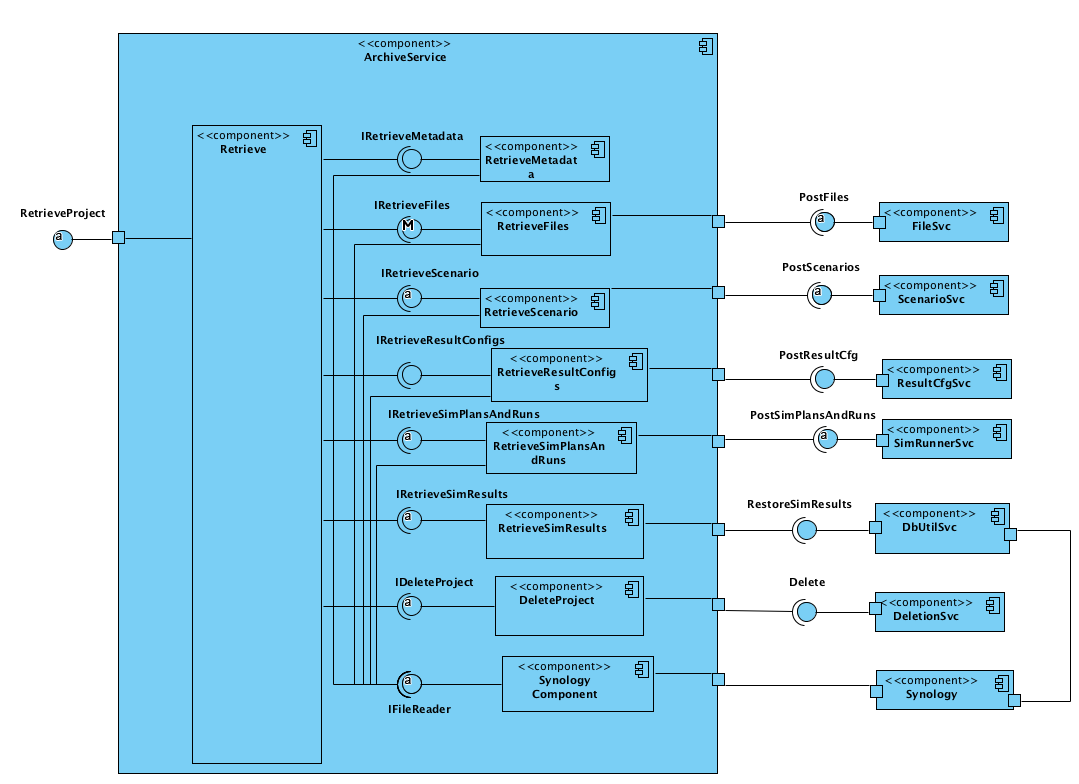
\includegraphics[scale=0.46]{grafiken/restoreComponent.png}
    \caption{Component Diagram for the Retrieve process}
    \label{fig:restore}
\end{figure}

The components RetrieveMetadata, Retrievefile, RetrieveScenarios, RetrieveResultCongfigs, and RetrieveSimulationPlansAndRuns have a common required interface
from the Synology component. Due to the fact that restoring needs the resources to be read from the Synology storage the interface (IFileReader) is required. 

\begin{figure}[H]
    \centering 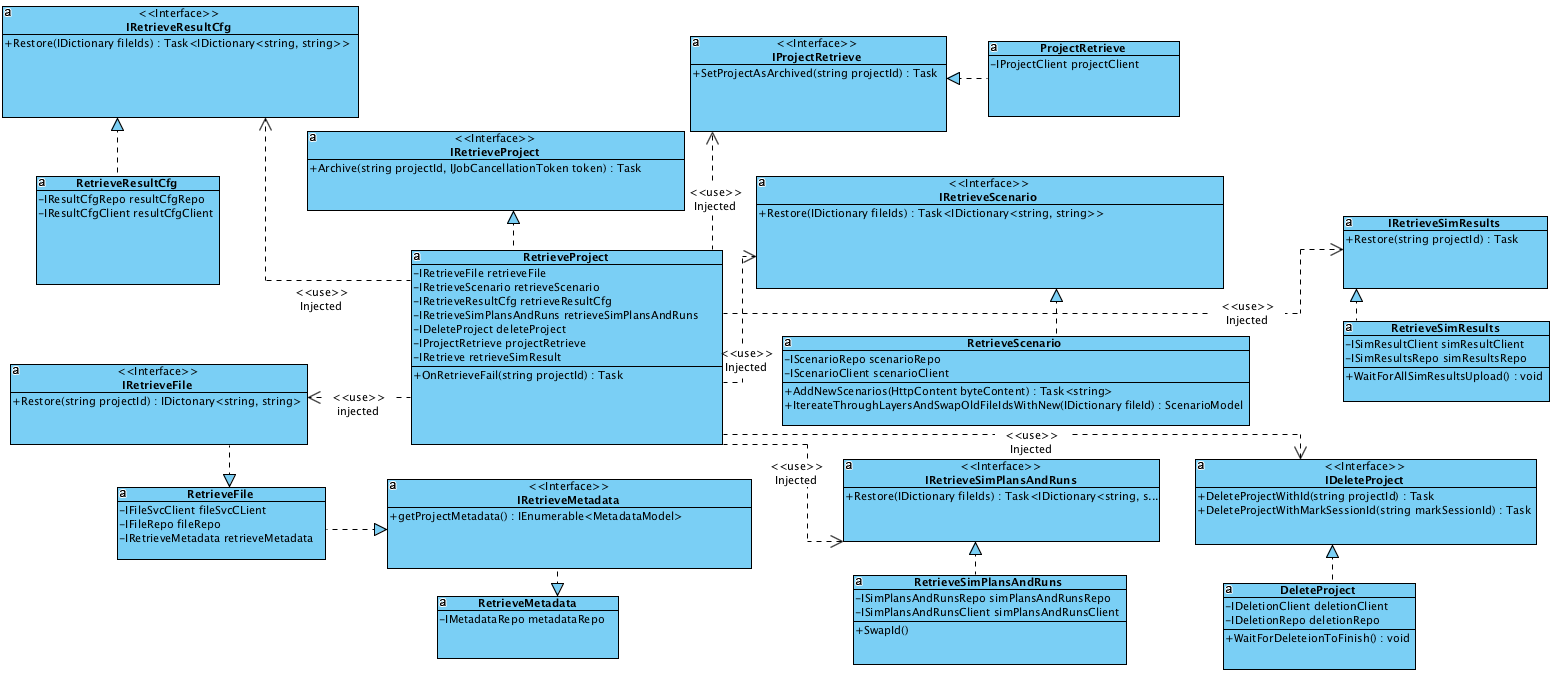
\includegraphics[height=6cm, angle=90, origin=c, width=10.5cm]{grafiken/restoreClass.png}
    \caption{Class Diagram for the Restore process (Top level)}
    \label{fig:restoreClass}
\end{figure}


Figure \ref{fig:restoreClass} illustrates the class digram for the retrieve process. The structure for the order of retrieve is very similar to the archive process
since it has to follow the MARS resource hierarchy (Section \ref{subsection:MARSResource}). All the dependencies for the retrieve project class are injected
using the Dependency Injection Container of .NET framework. The restoring is done by getting the data from the Synology and then posting it back to the system
using the respective service.

\subsection{Challenges}
\label{subsec:restoreProb}
Restoring the data back to the system is not so simple because it needs some additional work rather than just posting the data back to the system. 
The problem arises from the fact that the archived data has attributes like the resource id which is changed as a new resource is uploaded. For more clarification, 
Listing \ref{lst:marsMetadata} presents and example of an archived metadata. This resource is needed so that the restore process can determine the different 
attributes (e.g. title, project id) to ensure the contents of the resource would be the same as the archived data. During the file restore 
the file named KNPGIS.zip will 
be uploaded but the data id of the file would change as a new identifier is automatically assigned by the file service (See Listing \ref{lst:marsNewMetadata}). 
This is a big problem because the other 
resources such as scenarios, result configuration would now
depend on this new data id as the old data id is non existent in the MARS system. Listing \ref{lst:marsScenario} shows the archived scenario which has a reference 
to the data id from the archived resource. 
This is only one example as there are many attributes that must be taken care of. In oder to solve this the classes which are responsible
to post the corresponding data have a method which swaps these attributes. Listing \ref{lst:swapCode} shows an example of a method inside the RetrieveScenarios class.
The main task of this method is to dynamically get the contents as the scenarios are different for a particular model and then look for the new data id
that is assigned to a file after upload in the IDictionary map i.e. fileIds and replace the data id in the archived scenario. In conclusion, the mentioned problem
has been solved making a map of the old attribute and the new attribute and passing it to the child resource manager. The child searches for the new id using the 
old id as the key. Leading the attributes to be replaced with the correct new one, which allows a successful restore.

\newpage
\begin{lstlisting}[caption={Snippet of archived MARS metadata resource}, language=json,firstnumber=1, captionpos=b, label={lst:marsMetadata}]
{
    "DataId":"7cae6055-d7fd-418e-9ba0-bdc2980ffb4c",
    "Title":"KNPGIS.zip",
    "Description":null,
    "ProjectId":"c5deed87-dd03-45c3-a0c4-fdf9f1a307a0",
    "UserId":"af7e045f-edf4-4df5-a9c8-6327186e6ddb",
    "Privacy":"PROJECT_PRIVATE",
    "State":"TO_BE_DELETED"
}
\end{lstlisting}

\begin{lstlisting}[caption={Snippet of the uploaded MARS metadata resource}, language=json,firstnumber=1, captionpos=b, label={lst:marsNewMetadata}]
{
    "DataId":"27765261-8a65-45ab-bdeb-db8b5b7f8f43",
    "Title":"KNPGIS.zip",
    "Description":null,
    "ProjectId":"c5deed87-dd03-45c3-a0c4-fdf9f1a307a0",
    "UserId":"af7e045f-edf4-4df5-a9c8-6327186e6ddb",
    "Privacy":"PROJECT_PRIVATE",
    "State":"TO_BE_DELETED"
}
\end{lstlisting}

\begin{lstlisting}[caption={Snippet of the archived MARS scenario resource}, language=json,firstnumber=1, captionpos=b, label={lst:marsScenario}]
{
    "MetaDataId":"7cae6055-d7fd-418e-9ba0-bdc2980ffb4c",
    "Description":"No description available.",
    "ClearName":"gis_vector_percipitation.zip",
    "AllowedTypes":["SHAPEFILE","GEOJSON"],
    "ParameterMapping":[],"ValidationSuccessful":true},
}
\end{lstlisting}

\newpage
\begin{lstlisting}[language={[Sharp]C}, caption={A method in RetrieveScenarios to swap Attributes}, captionpos=b,label={lst:swapCode}]
private async Task<ScenarioModel> ItereateThroughLayersAndSwapOldFileIdsWithNew(IDictionary<string, string> fileIds, ScenarioModel dataScenarioModel)
{
    fileIds.TryGetValue(dataScenarioModel.ModelMetaData, out var newModelId);
    dataScenarioModel.ModelMetaData = newModelId;
    dataScenarioModel.ScenarioId = string.Empty;
    
    foreach (dynamic initializationDescriptionGeoPotentialFieldLayer in dataScenarioModel.InitializationDescription.GeoPotentialFieldLayers)
    {
        fileIds.TryGetValue((string)initializationDescriptionGeoPotentialFieldLayer["MetaDataId"], out var newGeoPotentialId);
        initializationDescriptionGeoPotentialFieldLayer["MetaDataId"] = newGeoPotentialId;
    }
}
\end{lstlisting}

Figure \ref{fig:sequenceRestore} illustrates the sequence diagram for the retrieve process. The starting step is similar to the archive process where a
check is made if a process for the project is running or not. If a process is found running then the restore process will be denied. The first after a
successful job creation is to fetch the metadata from the archives. Using the metadata the corresponding files are uploaded. After the file upload 
they need some more time to be processed. Therefore, the retrieve
also waits for the completion for the processing of all files.  This is an important step as it is required for the files to be in the FINISHED state
in order to create an scenario and result configurations.  As mentioned in
\ref{subsec:restoreProb} the necessary attributes would be swapped using the new model. Similarly, the simulation plan would be then uploaded followed
by the simulation runs. Lastly, the restore for the simulation results will be made. The retrieve process will come to halt after a finished
status of restore is received. 

\begin{figure}[H]
    \centering 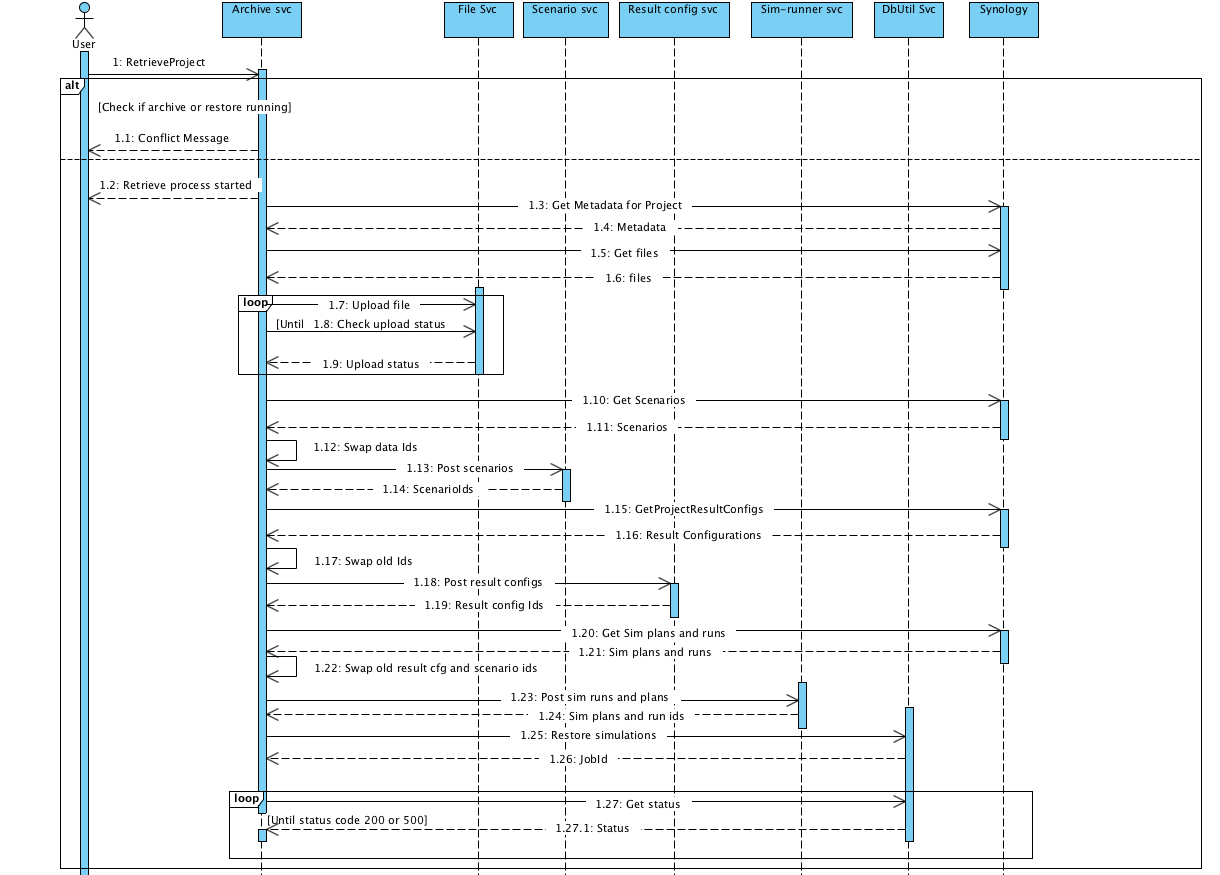
\includegraphics[scale=0.5, angle=90, origin=c]{grafiken/sequenceRestore.png}
    \caption{Sequence Diagram for the restore process}
    \label{fig:sequenceRestore}
\end{figure}

